\documentclass[tikz,border=12pt]{standalone}
% Shared visual language for standalone EMT block diagrams.
\usepackage{amsmath}
\usetikzlibrary{arrows.meta,backgrounds,calc,fit,positioning}

\tikzset{
    emt diagram/.style = {>={Stealth[length=2.4mm]}},
    line/.style        = {semithick, rounded corners=6pt},
    block/.style       = {draw, semithick, fill=white,
                          minimum height=1cm, minimum width=2.3cm},
    hblock/.style      = {block, minimum width=2.24cm, minimum height=1.3cm},
    vblock/.style      = {block, minimum width=1.3cm, minimum height=2.24cm},
    sum/.style         = {draw, semithick, fill=white, circle,
                          inner sep=2.6pt},
    signal/.style      = {circle, fill, inner sep=1.4pt,
                          label distance=3pt},
    sig/.style         = {font=\small},
    pm/.style          = {font=\scriptsize},
    wire jump/.style   = {line,
                          preaction={draw=white, line width=3pt,
                                     line cap=round}},
    enclosure/.style   = {draw, dashed, semithick, rounded corners=4pt},
    operator enclosure/.style = {enclosure, inner xsep=7mm, inner ysep=6mm}
}


% TUNABLES: command, limited-command return, and modulation rows.
\def\commandrow{1.2}
\def\returnrow{-1.2}
\def\striprow{0}
\def\anglerow{1.6}

\begin{document}

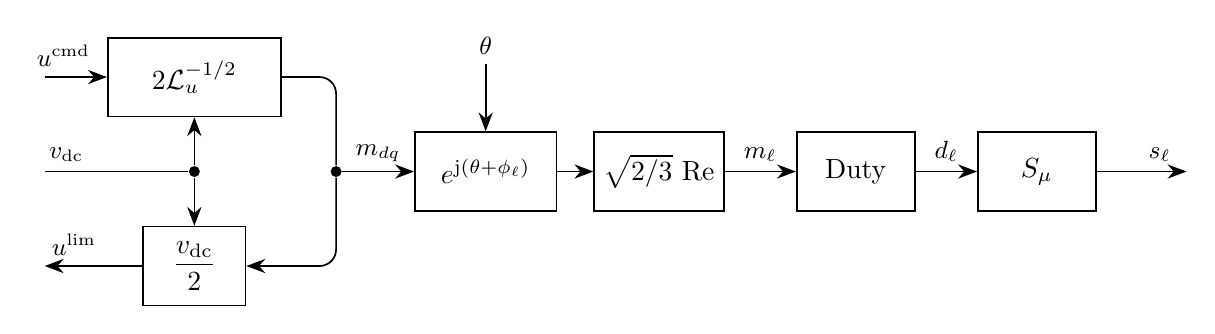
\begin{tikzpicture}[emt diagram]
% Voltage-command limit, DC normalization, phase projection, and
% carrier comparison; the limited command returns to the current controller.
\coordinate (origin) at (0,0);
\node[block, minimum width=2.2cm] (limit)
  at ($(origin)+(1.3,\commandrow)$) {$2\mathcal{L}_u^{-1/2}$};
\node[signal] (w) at ($(origin)+(3.1,\striprow)$) {};
\node[block, minimum width=1.3cm] (gain)
  at ($(origin)+(1.3,\returnrow)$) {$\dfrac{v_{\mathrm{dc}}}{2}$};
% dq signals denote complex pairs; the phase projection uses their real part.
\node[block, minimum width=1.8cm] (rotation)
  at ($(origin)+(5.0,\striprow)$) {$e^{\mathrm{j}(\theta+\phi_\ell)}$};
\node[block, minimum width=1.5cm] (projection)
  at ($(origin)+(7.2,\striprow)$) {$\sqrt{2/3}\,\operatorname{Re}$};
\node[block, minimum width=1.5cm] (duty)
  at ($(origin)+(9.7,\striprow)$) {Duty};
\node[block, minimum width=1.5cm] (switching)
  at ($(origin)+(12.0,\striprow)$) {$S_\mu$};
\draw[->, line] ($(origin)+(-0.6,\commandrow)$)
  -- node[sig, above, pos=0.3] {$u^{\mathrm{cmd}}$} (limit.west);
\draw[line] (limit.east) -| (w);
\draw[->, line] (w) -- node[sig, above] {$m_{dq}$} (rotation.west);
\draw[->, line] (rotation.east) -- (projection.west);
\draw[->, line] (projection.east) -- node[sig, above] {$m_\ell$} (duty.west);
\draw[->, line] (duty.east) -- node[sig, above] {$d_\ell$} (switching.west);
\draw[->, line] (switching.east)
  -- node[sig, above, pos=0.7] {$s_\ell$} ($(origin)+(13.9,\striprow)$);
\draw[->, line] (w) -- ($(origin)+(3.1,\returnrow)$) -- (gain.east);
\draw[->, line] (gain.west)
  -- node[sig, above, pos=0.7] {$u^{\mathrm{lim}}$}
  ($(origin)+(-0.6,\returnrow)$);

% DC-link voltage and frame angle inputs.
\node[signal] (vsplit) at ($(origin)+(1.3,\striprow)$) {};
\draw[line] ($(origin)+(-0.6,\striprow)$)
  -- node[sig, above, pos=0.15] {$v_{\mathrm{dc}}$} (vsplit);
\draw[->, line] (vsplit) -- (limit.south);
\draw[->, line] (vsplit) -- (gain.north);
\node[sig] (theta) at ($(origin)+(5.0,\anglerow)$) {$\theta$};
\draw[->, line] (theta.south) -- (rotation.north);

\end{tikzpicture}
\end{document}
